\documentclass[11pt]{article}

\usepackage[margin=1in]{geometry}
\usepackage{amsmath,amssymb,bm}
\usepackage{booktabs,array}
\usepackage{xcolor}
\usepackage{hyperref}
\usepackage{listings}
\usepackage{tikz}
\usetikzlibrary{arrows.meta,positioning}

\definecolor{codeblue}{RGB}{32,74,135}
\definecolor{codegreen}{RGB}{38,122,72}
\definecolor{back}{RGB}{247,248,250}
\hypersetup{colorlinks=true,linkcolor=codeblue,urlcolor=codeblue}
\lstset{
  language=Python,
  basicstyle=\ttfamily\small,
  keywordstyle=\color{codeblue}\bfseries,
  commentstyle=\color{codegreen},
  backgroundcolor=\color{back},
  frame=single,
  breaklines=true,
  showstringspaces=false,
  columns=fullflexible
}

\newcommand{\R}{\mathbb{R}}
\newcommand{\grad}{\nabla}

\title{PyTorch from Mathematical First Principles\\
\large Tensors, Automatic Differentiation, Optimizers, and \texttt{nn.Module}}
\author{Week 05 Study Notes --- Consciousness Project}
\date{\today}

\begin{document}
\maketitle
\tableofcontents
\newpage

\section{Purpose}

These notes explain the PyTorch ideas used to rebuild our causal-attention model. The goal is to connect
each command to mathematics already understood from the manual NumPy implementation. PyTorch does not
replace the chain rule; it records the computational graph and applies the chain rule automatically.

The central training cycle is
\[
\boxed{
\text{parameters}\longrightarrow\text{forward pass}\longrightarrow L
\longrightarrow\text{backward pass}\longrightarrow\text{parameter update}.
}
\]

\section{What PyTorch provides}

PyTorch is a Python library for multidimensional numerical arrays, automatic differentiation, neural-network
components, optimization, and accelerated computation on CPUs and GPUs. NumPy and PyTorch both support
vectors, matrices, indexing, and matrix multiplication. PyTorch additionally records operations involving
tracked tensors and can differentiate the final scalar loss with respect to all tracked parameters.

\section{Tensors}

A tensor is a multidimensional collection of numbers. In this setting it generalizes familiar objects:

\begin{center}
\begin{tabular}{lll}
\toprule
Object & Example shape & Interpretation\\
\midrule
Scalar & \texttt{()} & one number\\
Vector & \texttt{(d,)} & $d$ components\\
Matrix & \texttt{(n,d)} & $n$ rows and $d$ columns\\
Batch & \texttt{(B,n,d)} & $B$ matrices processed together\\
\bottomrule
\end{tabular}
\end{center}

Examples are:
\begin{lstlisting}
x = torch.tensor(3.0)
v = torch.tensor([1.0, 2.0, 3.0])
A = torch.tensor([[1.0, 2.0],
                  [3.0, 4.0]])
\end{lstlisting}

\subsection{Data types}

Continuous trainable parameters must use floating-point or complex values. Derivatives describe
infinitesimal changes, while an integer cannot change infinitesimally. Thus this is valid:
\begin{lstlisting}
x = torch.tensor(3.0, requires_grad=True)
\end{lstlisting}
but an integer tensor cannot require gradients.

Token IDs are discrete row addresses, so they use integer type:
\begin{lstlisting}
token_ids = torch.tensor([0, 1, 1, 2, 3], dtype=torch.long)
\end{lstlisting}
Here \texttt{torch.long} and \texttt{torch.int64} name the same 64-bit integer type. We differentiate the
embedding values selected by these IDs, not the IDs themselves.

\section{CPU and GPU}

A CPU is a general-purpose processor with a relatively small number of powerful cores. It handles
sequential and logically varied work well. A GPU has many parallel arithmetic units and is effective for
large, regular calculations such as matrix multiplication.

Every tensor lives on a device. A tensor created normally is on the CPU:
\begin{lstlisting}
print(x.device)  # cpu
\end{lstlisting}
NVIDIA GPUs are commonly accessed through CUDA; Apple Silicon GPUs can be accessed through MPS. Tensors
used in one operation must normally share a device. Moving data also has a cost, so our tiny model is more
appropriate for the CPU even though large neural networks benefit strongly from GPU parallelism.

\section{Automatic differentiation}

\subsection{Tracking a variable}

Consider
\[
L=(x-5)^2,qquad x=3.
\]
Creating $x$ with \texttt{requires\_grad=True} tells PyTorch to record operations involving $x$:
\begin{lstlisting}
x = torch.tensor(3.0, requires_grad=True)
loss = (x - 5) ** 2
\end{lstlisting}
The forward pass evaluates $L=4$ and records
\[
x\longrightarrow u=x-5\longrightarrow L=u^2.
\]
At this point \texttt{x.grad} is still \texttt{None}; the graph has been recorded, but differentiation has
not yet been requested.

\subsection{The backward command}

The command
\begin{lstlisting}
loss.backward()
\end{lstlisting}
starts at the scalar loss and traverses the graph in reverse. Mathematically,
\[
\frac{\partial L}{\partial x}
=\frac{\partial L}{\partial u}\frac{\partial u}{\partial x}
=2u(1)=2(x-5)=-4.
\]
PyTorch stores this result in \texttt{x.grad}. It does not use finite differences; it uses local derivative
rules and reverse-mode chain-rule composition.

\subsection{Vector and matrix gradients}

If $x\in\R^d$ and $L$ is scalar, then \texttt{x.grad} has the same shape as $x$:
\[
\grad_xL=
\begin{bmatrix}
\partial L/\partial x_1\\
\vdots\\
\partial L/\partial x_d
\end{bmatrix}.
\]
For $L=\sum_i x_i^2$,
\[
\grad_xL=2x.
\]

For $Z=XW$ and $L=\sum_{ij}Z_{ij}^2$,
\[
\grad_WL=X^\top(2Z).
\]
This has the same structure as our vocabulary-projection result
\[
\grad_{W_{\rm vocab}}L=O^\top G.
\]

\subsection{Gradient accumulation}

PyTorch adds new gradient contributions to the existing \texttt{.grad}. If
\[
L_1=x^2,\qquad L_2=(x-5)^2,qquad x=3,
\]
then calling backward on both losses without clearing gives
\[
x.\mathrm{grad}=6+(-4)=2.
\]
This is useful when several paths or mini-batches contribute to one parameter. Ordinary gradient descent,
however, needs the gradient at the current parameter state, so old iteration gradients must be cleared.

\section{The PyTorch attention forward pass}

Our tracked parameters are
\[
E,\quad W_Q,\quad W_K,\quad W_V,\quad W_{\rm vocab}.
\]
Integer token IDs select embedding rows:
\[
X=E[\text{token IDs}].
\]
PyTorch records the indexing operation, so repeated occurrences of one ID automatically accumulate into
the corresponding row of $E.\mathrm{grad}$.

The attention calculation is unchanged:
\begin{align}
Q&=XW_Q,&K&=XW_K,&V&=XW_V,\\
S&=\frac{QK^\top}{\sqrt{d_k}}+M,&A&=\operatorname{softmax}(S,\mathrm{dim}=1),\\
O&=AV,&Z&=O_{\rm train}W_{\rm vocab}.
\end{align}

The causal mask contains zero on and below the diagonal and $-\infty$ above it. Since
$e^{-\infty}=0$, blocked future positions receive zero attention probability.

\section{Cross-entropy}

PyTorch's functional interface supplies:
\begin{lstlisting}
import torch.nn.functional as F
loss = F.cross_entropy(logits, target_ids)
\end{lstlisting}
For logits $Z\in\R^{N\times |\mathcal V|}$ and one correct class ID $t_i$ per row, this computes
\[
L=-\frac1N\sum_{i=1}^N\log
\frac{e^{Z_{i,t_i}}}{\sum_j e^{Z_{ij}}}.
\]
Raw logits, rather than softmax probabilities, must be passed to \texttt{F.cross\_entropy}; the function
combines a numerically stable log-softmax with negative log-likelihood.

One call to \texttt{loss.backward()} then reproduces our manually derived gradients for all parameters.
The small discrepancy between NumPy values near $10^{-17}$ and PyTorch values near $10^{-8}$ came from
NumPy's typical 64-bit floats versus PyTorch's default 32-bit floats.

\section{Optimizers and the training loop}

Stochastic gradient descent implements
\[
\theta_{k+1}=\theta_k-\eta\grad_\theta L(\theta_k).
\]
An optimizer holds references to the exact parameter objects supplied to it:
\begin{lstlisting}
optimizer = torch.optim.SGD(parameters, lr=0.1)
\end{lstlisting}
Recreating parameter tensors requires recreating the optimizer; an old optimizer continues to point to
the old tensor objects.

The three central training commands are:
\begin{lstlisting}
optimizer.zero_grad()  # clear previous iteration gradients
loss.backward()        # calculate current gradients
optimizer.step()       # update parameters
\end{lstlisting}

The full conceptual loop is:
\begin{enumerate}
\item clear old gradients;
\item run a fresh forward pass using current parameters;
\item calculate the scalar loss;
\item run backpropagation;
\item update all parameters;
\item record \texttt{loss.item()} for plotting.
\end{enumerate}

A fresh forward pass is necessary because parameter values change and PyTorch normally releases the old
computational graph after backward. Reusing a derived tensor such as $X=E[\text{IDs}]$ across iterations
would reuse stale values and an already-freed graph.

\section{Why use \texttt{nn.Module}?}

Our first PyTorch implementation stored five unrelated global tensors. An \texttt{nn.Module} groups model
parameters and the forward rule into one object. This provides consistent parameter registration, optimizer
construction, device movement, saving, loading, and composition with other layers.

\subsection{Class structure}

\begin{lstlisting}
class ToyAttentionModel(nn.Module):

    def __init__(self):
        super().__init__()
        # Define persistent trainable parameters.

    def forward(self, token_ids):
        # Convert input token IDs into logits.
        return logits
\end{lstlisting}

\texttt{self} means the particular model object being constructed or used. If the class assigns
\texttt{self.E}, the instantiated object exposes \texttt{model.E}.

\texttt{super().\_\_init\_\_()} initializes the machinery inherited from \texttt{nn.Module}. The parentheses
matter: naming a method refers to it, while adding parentheses calls it.

\subsection{Registered parameters}

Inside a module,
\begin{lstlisting}
self.E = nn.Parameter(torch.tensor(...))
\end{lstlisting}
creates a tracked tensor and registers it as model state. Registered parameters appear in
\texttt{model.parameters()} and \texttt{model.named\_parameters()}.

For our toy model, the registered shapes are:
\begin{center}
\begin{tabular}{lc}
\toprule
Parameter & Shape\\
\midrule
$E$ & $(4,4)$\\
$W_Q$ & $(4,2)$\\
$W_K$ & $(4,2)$\\
$W_V$ & $(4,3)$\\
$W_{\rm vocab}$ & $(3,4)$\\
\bottomrule
\end{tabular}
\end{center}

The optimizer can therefore be constructed with
\begin{lstlisting}
optimizer = torch.optim.SGD(model.parameters(), lr=0.1)
\end{lstlisting}
without explicitly listing each matrix.

\subsection{What belongs in \texttt{forward}?}

The forward method should map inputs to model outputs:
\[
\text{token IDs}\longrightarrow\text{logits}.
\]
The target IDs, loss, gradient clearing, backward call, and optimizer step belong to the external training
procedure. This separation allows the same model to be used for training, validation, and inference.

Calling
\begin{lstlisting}
logits = model(token_ids)
\end{lstlisting}
automatically invokes \texttt{model.forward(token\_ids)}. The model should return logits; the training loop
compares them with targets.

\section{Computational graph picture}

\begin{figure}[ht]
\centering
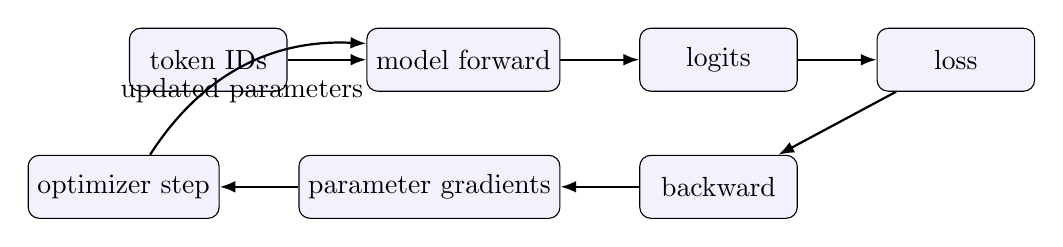
\begin{tikzpicture}[node distance=8mm and 10mm,
box/.style={draw,rounded corners,fill=blue!5,minimum width=20mm,minimum height=8mm},
arr/.style={-{Latex[length=2mm]},thick}]
\node[box] (ids) {token IDs};
\node[box,right=of ids] (model) {model forward};
\node[box,right=of model] (logits) {logits};
\node[box,right=of logits] (loss) {loss};
\node[box,below=of logits] (back) {backward};
\node[box,left=of back] (grads) {parameter gradients};
\node[box,left=of grads] (step) {optimizer step};
\draw[arr] (ids)--(model); \draw[arr] (model)--(logits); \draw[arr] (logits)--(loss);
\draw[arr] (loss)--(back); \draw[arr] (back)--(grads); \draw[arr] (grads)--(step);
\draw[arr] (step) to[bend left=30] node[below] {updated parameters} (model);
\end{tikzpicture}
\caption{Training repeatedly builds a forward graph, backpropagates through it, and updates the registered parameters.}
\end{figure}

\section{Common errors and their meanings}

\begin{description}
\item[\texttt{NameError: name 'x' is not defined}] The defining cell did not run in the current kernel. Notebook
variables follow execution order, not visual order.

\item[Integer tensor cannot require gradients] Use floating-point values for continuous trainable parameters.
Keep token IDs as integer tensors without gradients.

\item[\texttt{.grad} is \texttt{None}] The tensor did not participate in the loss graph, did not require gradients,
or backward was not called. A zero tensor means a calculated derivative of zero; \texttt{None} means no gradient
was calculated for that object.

\item[Calling \texttt{loss.backward} without parentheses] This merely refers to the method. Use
\texttt{loss.backward()} to execute it.

\item[Backward through the graph a second time] A derived tensor from an old forward pass was reused. Recompute
the forward pass with current parameters.

\item[Training behaves erratically] Check that \texttt{optimizer.zero\_grad()} occurs once per iteration before
backward and that the optimizer references the current parameter objects.

\item[Code after \texttt{return} does not run] Returning exits the method immediately. Model creation and training
must be outside the class and unindented.

\item[Model ignores its input] Do not overwrite a \texttt{forward} argument with a hard-coded tensor inside the
method.
\end{description}

\section{Notebook execution discipline}

A notebook stores code and displayed outputs, but a restarted kernel loses Python memory. A reliable workflow is:
\begin{enumerate}
\item place imports and reusable definitions near the beginning;
\item keep expensive experiments later;
\item use ``Restart Kernel and Run All'' to reveal stale-variable dependencies;
\item move mature reusable functions into a Python module when the notebook becomes long.
\end{enumerate}

\section{Learning from random initialization}

The first toy model began with matrices whose entries were chosen by hand. That is useful for checking every
calculation, but a trainable model should not depend on already favorable weights. We therefore repeated the
same experiment with randomly initialized parameters and verified that gradient descent still reduced the
cross-entropy loss.

\subsection{Architecture sizes are hyperparameters}

The integers
\[
  V=\texttt{vocab\_size},\qquad d_{\rm model},\qquad d_k,\qquad d_v
\]
describe the architecture. They are selected deliberately rather than sampled randomly. They determine the
parameter shapes:
\begin{center}
\begin{tabular}{lll}
\toprule
Parameter & Shape & Role\\
\midrule
$E$ & $(V,d_{\rm model})$ & token embedding table\\
$W_Q$ & $(d_{\rm model},d_k)$ & query projection\\
$W_K$ & $(d_{\rm model},d_k)$ & key projection\\
$W_V$ & $(d_{\rm model},d_v)$ & value projection\\
$W_{\rm vocab}$ & $(d_v,V)$ & hidden state to vocabulary logits\\
\bottomrule
\end{tabular}
\end{center}
For the experiment, $(V,d_{\rm model},d_k,d_v)=(4,4,2,3)$. The resulting logit matrix has shape $(4,4)$:
four supervised positions and four possible next-token classes.

\subsection{Reproducible pseudorandom numbers}

The command
\begin{lstlisting}
torch.manual_seed(0)
\end{lstlisting}
sets the initial state of PyTorch's pseudorandom-number generator. The values are still varied, but rerunning
the program with the same seed generates the same sequence. This makes an experiment reproducible. Changing
the seed changes the initial weights and may change the precise learning curve.

\subsection{Why scale random weights?}

A matrix product forms each output coordinate by adding $d_{\rm in}$ terms. If all weights have unit variance,
the variance of this sum can grow roughly in proportion to $d_{\rm in}$. Large activations can make optimization
unstable or push nonlinearities into saturated regimes. A simple initialization is therefore
\[
  W_{ij}\sim\frac{\mathcal N(0,1)}{\sqrt{d_{\rm in}}}.
\]
The factor $1/\sqrt{d_{\rm in}}$ keeps the initial output scale roughly independent of the input dimension.
In our model this gives
\begin{align*}
 E&=\frac{\operatorname{randn}(V,d_{\rm model})}{\sqrt{d_{\rm model}}},\\
 W_Q,W_K,W_V&=\frac{\operatorname{randn}(\cdot,\cdot)}{\sqrt{d_{\rm model}}},\\
 W_{\rm vocab}&=\frac{\operatorname{randn}(d_v,V)}{\sqrt{d_v}}.
\end{align*}
This initialization scaling is conceptually separate from the attention-score scaling
$QK^\top/\sqrt{d_k}$. The former controls the scale of newly created parameters; the latter controls dot-product
scores during every forward pass.

\subsection{What \texttt{nn.Parameter} means}

An \texttt{nn.Parameter} is a tensor that an enclosing \texttt{nn.Module} registers as trainable. For example,
\begin{lstlisting}
self.W_Q = nn.Parameter(
    torch.randn(d_model, d_k) / (d_model ** 0.5)
)
\end{lstlisting}
has three consequences:
\begin{enumerate}
  \item it behaves like a tensor in expressions such as \texttt{X @ self.W\_Q};
  \item it tracks derivatives, so backpropagation stores $\partial L/\partial W_Q$ in
  \texttt{self.W\_Q.grad};
  \item it appears in \texttt{model.parameters()} and \texttt{model.named\_parameters()}, so an optimizer can
  discover and update it.
\end{enumerate}
A regular tensor assigned to the module is not automatically a trainable registered parameter. Also, the
scaling must occur inside the constructor:
\begin{lstlisting}
# Correct: the object assigned to self.W_Q is a Parameter.
self.W_Q = nn.Parameter(torch.randn(d_model, d_k) / d_model**0.5)
\end{lstlisting}

\subsection{Randomly initialized module}

The essential initialization is:
\begin{lstlisting}
class ToyAttentionModel(nn.Module):
    def __init__(self, vocab_size, d_model, d_k, d_v):
        super().__init__()

        self.E = nn.Parameter(
            torch.randn(vocab_size, d_model) / d_model**0.5
        )
        self.W_Q = nn.Parameter(
            torch.randn(d_model, d_k) / d_model**0.5
        )
        self.W_K = nn.Parameter(
            torch.randn(d_model, d_k) / d_model**0.5
        )
        self.W_V = nn.Parameter(
            torch.randn(d_model, d_v) / d_model**0.5
        )
        self.W_vocab = nn.Parameter(
            torch.randn(d_v, vocab_size) / d_v**0.5
        )
\end{lstlisting}
The forward computation remains unchanged: embedding lookup, query/key/value projections, scaled causal
attention, value aggregation, and vocabulary logits. Cross-entropy and optimization remain outside
\texttt{forward}.

\subsection{What the experiment establishes}

The loss decreased smoothly from a random starting point, and every registered parameter had its intended
shape. This shows that the forward graph, automatic differentiation, and optimizer are connected correctly,
and that learning does not depend on the earlier hand-selected matrices. Because the training data is still
one tiny sequence, a very small training loss demonstrates successful optimization and memorization rather
than general language ability. Generalization must be evaluated on held-out sequences.

\section{Review questions}

Answer these without running code:
\begin{enumerate}
\item What extra capability does a tracked PyTorch tensor provide beyond a NumPy array?
\item Why can token IDs use integers while trainable weights require floats?
\item What is recorded during the forward pass?
\item What exactly does \texttt{loss.backward()} do?
\item Why does a parameter gradient have the same shape as the parameter?
\item Why do gradients accumulate, and why must a training loop clear them?
\item What is the distinction between backpropagation and an optimizer step?
\item Why must the forward pass be recomputed after every parameter update?
\item What is the purpose of \texttt{nn.Parameter}?
\item Why should cross-entropy and target IDs usually remain outside \texttt{forward}?
\item Why does \texttt{model.parameters()} simplify optimizer construction?
\item What is the difference between a zero gradient and \texttt{None}?
\item Which dimensions are architecture choices, and which quantities are randomly initialized?
\item What does \texttt{torch.manual\_seed(0)} guarantee, and what does it not guarantee?
\item Why divide a random matrix by the square root of its input dimension?
\item Why must scaling occur inside \texttt{nn.Parameter(...)}?
\end{enumerate}

\section{Next steps}

The next session should begin by reconstructing the randomly initialized class from a blank cell. Then we can:
\begin{enumerate}
\item compare several seeds and learning rates without changing the model equations;
\item compare selected autograd derivatives with centered finite differences;
\item replace manual parameter matrices with \texttt{nn.Embedding} and \texttt{nn.Linear};
\item add positional encoding and test sensitivity to word order;
\item train on multiple sequences and measure held-out loss.
\end{enumerate}

\end{document}
